\documentclass[nonacm]{acmart}
\settopmatter{printfolios=true,printccs=true,printacmref=true}

\usepackage{mathtools}
\usepackage{amsmath}
\usepackage{cleveref}

%%
%% Macros
%%
%%
%% Terms
%%
\newcommand{\lit}[1]{\ensuremath{\ulcorner #1 \urcorner}}
\newcommand{\cut}[2]{\ensuremath{\langle #1 \mid #2 \rangle}}
\newcommand{\done}{\ensuremath{\mathbf{done}}}
\newcommand{\ifz}[3]{\ensuremath{\mathbf{ifz}(#1, #2, #3)}}
\newcommand{\letin}[3]{\ensuremath{\mathbf{let}\ #1 = #2\ \mathbf{in}\ #3}}
\newcommand{\caseof}[2]{\ensuremath{\mathbf{case}\ #1\ \mathbf{of}\ \{ #2 \}}}
\newcommand{\case}[1]{\ensuremath{\mathbf{case}\ \{ #1 \}}}
\newcommand{\cocase}[1]{\ensuremath{\mathbf{cocase}\ \{ #1 \}}}
\newcommand{\goto}[2]{\ensuremath{\mathbf{goto}(#1; #2)}}
\newcommand{\lab}[2]{\ensuremath{\mathbf{label}\ #1\ \{#2 \}}}
\newcommand{\defi}[2]{\ensuremath{\mathbf{def}\ #1 \coloneq #2}}

%%
%% AxCut Terms
%%
\newcommand{\jump}[1]{\ensuremath{\mathbf{jump}\, #1}}
\newcommand{\invoke}[2]{\ensuremath{\mathbf{invoke}\, #1\, #2}}
\newcommand{\switch}[2]{\ensuremath{\mathbf{switch}\, #1\, #2}}
\newcommand{\substitute}[2]{\ensuremath{\mathbf{substitute}[#1];#2}}
\newcommand{\letac}[3]{\ensuremath{\mathbf{let}\, #1 = #2; #3}}
\newcommand{\new}[3]{\ensuremath{\mathbf{new}\, #1 = #2; #3}}
\newcommand{\bra}[1]{\ensuremath{\{ #1 \}}}
\newcommand{\ifzac}[3]{\ensuremath{\mathbf{ifz}(#1)\{ () \Rightarrow #2, () \Rightarrow #3 \}}}
\newcommand{\litac}[3]{\ensuremath{\mathbf{lit}[\lit{#1}]\{ #2 \Rightarrow #3 \}}}
\newcommand{\opac}[3]{\ensuremath{\odot(#1)\{ #2 \Rightarrow #3 \}}}

%%
%% Languages and Calculi
%%
\newcommand{\lambdamumu}{$\lambda\mu\tilde\mu$-calculus}
\newcommand{\surfacelang}{\textbf{Fun}}
\newcommand{\targetlang}{\textbf{Core}}
\newcommand{\machinelang}{\textbf{AxCut}}

%%
%% Types / Typing Rules / Typing Contexts
%%
\newcommand{\tyint}{\mathbf{Int}}
\newcommand{\wrap}[1]{:^{\text{\tiny#1}}}
\newcommand{\prd}{\wrap{prd}}
\newcommand{\cnt}{\wrap{cns}}
\newcommand{\wellformed}[1]{#1\ \textsc{Ok}}
\newcommand{\data}[2]{\mathbf{data}\, \mathtt{#1}\, \{ #2 \}}
\newcommand{\codata}[2]{\mathbf{codata}\, \mathtt{#1}\, \{ #2 \}}

%%
%% Evaluation / Reduction / Operational Semantics
%%
\newcommand{\reducesto}{\ensuremath{\triangleright}}


%%
%% Translations / Transfomations
%%
\newcommand{\focus}[1]{\ensuremath{\mathcal{F}(#1)}}
\newcommand{\name}[1]{\ensuremath{\mathcal{N}(#1)}}
\newcommand{\bind}[2]{\ensuremath{\mathsf{bind}(#1)[#2]}}
\newcommand{\redundancy}[1]{\ensuremath{\mathcal{R}(#1)}}
\newcommand{\fresh}[1]{\ensuremath{(#1\text{ fresh})}}
\newcommand{\translate}[1]{\ensuremath{\llbracket #1 \rrbracket}}
\newcommand{\translatestar}[2]{\ensuremath{\llbracket #1 \rrbracket_{#2}^{\ast}}}


\begin{document}
%%
%% Title information
%%
\title{Compiling Functional Languages To Machine Code}
\subtitle{A Complete Story}

%%
%% Keywords
%%
\keywords{Intermediate representations, continuations, codata types, control effects}

%%
%% CCS Classification
%%

\begin{CCSXML}
  <ccs2012>
     <concept>
         <concept_id>10003752.10003753.10003754.10003733</concept_id>
         <concept_desc>Theory of computation~Lambda calculus</concept_desc>
         <concept_significance>500</concept_significance>
         </concept>
     <concept>
         <concept_id>10011007.10011006.10011041</concept_id>
         <concept_desc>Software and its engineering~Compilers</concept_desc>
         <concept_significance>500</concept_significance>
         </concept>
     <concept>
         <concept_id>10011007.10011006.10011008.10011024.10011027</concept_id>
         <concept_desc>Software and its engineering~Control structures</concept_desc>
         <concept_significance>300</concept_significance>
         </concept>
   </ccs2012>
\end{CCSXML}
  
\ccsdesc[500]{Theory of computation~Lambda calculus}
\ccsdesc[500]{Software and its engineering~Compilers}
\ccsdesc[300]{Software and its engineering~Control structures}

%%
%% Author: David Binder
%%
\author{David Binder}
\orcid{0000-0003-1272-0972}
\affiliation{
  \department{Department of Computer Science}
  \institution{University of Tübingen}
  \city{Tübingen}
  \country{Germany}
}
\email{david.binder@uni-tuebingen.de}

%%
%% Author: Marco Tzschentke
%%
\author{Marco Tzschentke}
\orcid{0009-0004-8834-2984}
\affiliation{
  \department{Department of Computer Science}
  \institution{University of Tübingen}
  \city{Tübingen}
  \country{Germany}
}
\email{marco.tzschentke@uni-tuebingen.de}

%%
%% Author: Marius Müller
%%
\author{Marius Müller}
\orcid{0000-0002-0260-6298}
\affiliation{
  \department{Department of Computer Science}
  \institution{University of Tübingen}
  \city{Tübingen}
  \country{Germany}
}
\email{mari.mueller@uni-tuebingen.de}

%%
%% Author: Philipp Schuster
%%
\author{Philipp Schuster}
\orcid{0000-0001-8011-0506}
\affiliation{
  \department{Department of Computer Science}
  \institution{University of Tübingen}
  \city{Tübingen}
  \country{Germany}
}
\email{philipp.schuster@uni-tuebingen.de}

%%
%% Author: Jonathan Immanuel Brachthäuser
%%
\author{Jonathan Immanuel Brachthäuser}
\orcid{0000-0001-9128-0391}
\affiliation{
  \department{Department of Computer Science}
  \institution{University of Tübingen}
  \city{Tübingen}
  \country{Germany}
}
\email{jonathan.brachthaeuser@uni-tuebingen.de}

%%
%% Author: Klaus Ostermann
%%
\author{Klaus Ostermann}
\orcid{0000-0001-5294-5506}
\affiliation{
  \department{Department of Computer Science}
  \institution{University of Tübingen}
  \city{Tübingen}
  \country{Germany}
}
\email{klaus.ostermann@uni-tuebingen.de}

%%
%% Abstract
%%
\begin{abstract}
  Compiling a high-level functional programming language to machine code that can be executed efficiently on a modern machine is a complicated task, since we have to traverse many different levels of abstraction.
  In this paper we tell the complete story, starting from a ML-like functional programming language and ending up with Risc-V and x86-64 machine code.
  The novelty of our approach lies in the fact that we use the sequent calculus, and sequent calculus inspired languages, in specifying the intermediate stages of our compiler.
\end{abstract}

\maketitle

%%
%% Section: Introduction
%%
\section{Introduction}
\label{sec:introduction}
Compiling a modern functional programming language like Haskell or OCaml to efficient machine code is a complicated affair, since we have to cross many different levels of abstraction in order to bridge the gap between high-level conveniences and low-level concerns.
In this paper we present such a complete compilation pipeline, starting with a surface language which supports different calling conventions, codata types and control effects, and ending up with machine code for Risc-V and X86-64.
More concretely, we show how to implement all of the following stages in the compiler pipeline:
\medskip

\begin{center}
  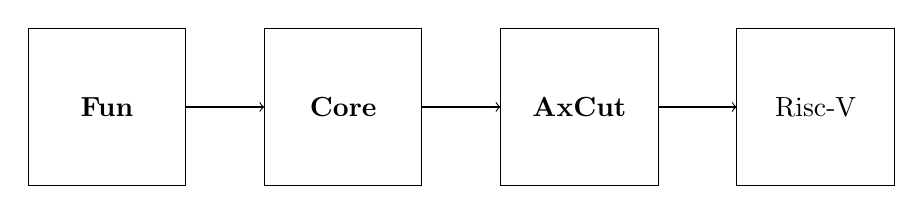
\begin{tikzpicture}
    \draw (0,0) rectangle (2,2) node[pos=.5] {\surfacelang};
    \draw (3,0) rectangle (5,2) node[pos=.5] {\targetlang};
    \draw (6,0) rectangle (8,2) node[pos=.5] {\machinelang};
    \draw (9,0) rectangle (11,2) node[pos=.5] {Risc-V};
    \draw[->] (2,1) -- (3,1);
    \draw[->] (5,1) -- (6,1);
    \draw[->] (8,1) -- (9,1);
  \end{tikzpicture}
\end{center}

The rest of this article is structured as follows:
\begin{itemize}
    \item In \cref{sec:fun} we introduce the surface language \surfacelang.
    \item In \cref{sec:core} we introduce the intermediate language \targetlang.
    \item In \cref{sec:translation} we show how to translate programs from the surface language \surfacelang\ to the intermediate language \targetlang.
    \item In \cref{sec:naming-transformation} we show a transformation on programs in \targetlang\ which names all intermediate computations, similar to ANF or focusing transformations.
    \item In \cref{sec:redundancy-elimination} and \cref{sec:substructurality-analysis} we \ldots
    \item In \cref{sec:axcut} we introduce the low-level intermediate language \machinelang, and in \cref{sec:toaxcut} we show how to compile \targetlang\ to \machinelang.
\end{itemize}
We discuss related work in \cref{sec:related-work} and conclude in \cref{sec:conclusion}.


%%
%% Section: The Surface Language Fun
%%
\section{The Surface Language Fun}
\label{sec:fun}
\begin{definition}[Syntactic Conventions]
    We use the following metavariables for all languages:
    \[
      \begin{array}{rcll}
        K & \coloneqq & \mathtt{Nil}, \mathtt{Cons}, \mathtt{Tup} & \emph{Constructors}\\
        D & \coloneqq & \mathtt{hd}, \mathtt{tl}, \mathtt{fst}, \mathtt{snd} & \emph{Destructors}\\
        \odot  & \coloneqq & + \mid - \mid * & \emph{Arithmetic Operators}
      \end{array}
    \]
  \end{definition}
  
  \begin{definition}[Syntax of Fun]
    \[ 
      \begin{array}{r c l l}
        t & \coloneqq & x \mid \lit{n} \mid t \odot t \mid \ifz{t}{t}{t} \mid \letin{x}{t}{t} \mid f(\overline{t}; \overline{\alpha}) & \emph{Terms}\\
        & \mid & K(\overline{t}) \mid \caseof{t}{\overline{K(\overline{x}) \Rightarrow t}} \mid t.D(\overline{t}) \mid \cocase{\overline{D(\overline{x}) \Rightarrow t}} & \\
        & \mid & \lambda x.t \mid t\ t \mid \lab{\alpha}{t} \mid \goto{t}{\alpha} & \\
        \Theta & \coloneqq & \emptyset \mid \defi{f(\overline{x};\overline{\alpha})}{t}; \Theta & \emph{Programs}\\
      \end{array}
    \]
  \end{definition}

%%
%% Subsec: Typing Rules
%%
\subsection{Typing Rules}
\label{subsec:fun:typing-rules}

\begin{definition}[Types and Typing Contexts]
  \[
    \begin{array}{l c l r}
      \tau   & \Coloneqq & \tyint \mid \mathtt{List}(\tau) \mid \mathtt{Pair}(\tau,\tau) \mid \mathtt{Stream}(\tau)\ \mid\ \mathtt{LPair}(\tau,\tau) \mid \tau \to \tau & \emph{Types}\\
      \Gamma & \Coloneqq & \emptyset \mid \Gamma, x \prd \tau \mid \Gamma, \alpha \cnt \tau & \emph{Typing Contexts}
    \end{array}
  \]
\end{definition}

\begin{minipage}{\textwidth}
  \begin{minipage}{0.3\textwidth}
    \begin{prooftree}
      \AxiomC{$x \prd \tau \in \Gamma$}
      \RightLabel{\textsc{Var}}
      \UnaryInfC{$\Gamma \vdash x : \tau$}
    \end{prooftree}
  \end{minipage}
  \hfill
  \begin{minipage}{0.3\textwidth}
    \begin{prooftree}
      \AxiomC{\phantom{$x : \tau \in \Gamma$}}
      \RightLabel{\textsc{Lit}}
      \UnaryInfC{$\Gamma \vdash \lit{n}:\tyint$}
    \end{prooftree}
  \end{minipage}
  \hfill
  \begin{minipage}{0.3\textwidth}
    \begin{prooftree}
      \AxiomC{$\Gamma \vdash t_1: \tyint \quad \Gamma \vdash t_2: \tyint$}
      \RightLabel{\textsc{Op}}
      \UnaryInfC{$\Gamma \vdash t_1\odot t_2 : \tyint$}
    \end{prooftree}
  \end{minipage}
  \hfill
  \vspace{1em}

  \begin{minipage}{0.55\textwidth}
    \begin{prooftree}
      \AxiomC{$\Gamma \vdash n : \tyint$}
      \AxiomC{$\Gamma \vdash t_1 : \tau$}
      \AxiomC{$\Gamma \vdash t_2 : \tau$}
      \RightLabel{\textsc{Ifz}}
      \TrinaryInfC{$\Gamma \vdash \ifz{n}{t_1}{t_2} : \tau$}
    \end{prooftree}
  \end{minipage}
  \hfill
  \begin{minipage}{0.4\textwidth}
    \begin{prooftree}
      \AxiomC{$\Gamma \vdash t_1 : \tau_1$}
      \AxiomC{$\Gamma, x \prd \tau_1 \vdash t_2 : \tau_2$}
      \RightLabel{\textsc{Let}}
      \BinaryInfC{$\Gamma \vdash \letin{x}{t_1}{t_2} :\tau_2$}
    \end{prooftree}
  \end{minipage}
  \hfill
  \vspace{1em}

  \begin{minipage}{\textwidth}
    \begin{prooftree}
      \AxiomC{$\mathbf{def}\ f(\overline{x_i \prd \tau_i};\overline{\alpha_j\cnt\tau_j}) :\tau \in P$}
      \AxiomC{$\overline{\Gamma \vdash t_i : \tau_i}$}
      \AxiomC{$\overline{\beta_j \cnt \tau_j \in \Gamma}$}
      \RightLabel{\textsc{Call}}
      \TrinaryInfC{$\Gamma \vdash f(\overline{t_i};\overline{\beta_j}) : \tau$}
    \end{prooftree}
  \end{minipage}
  \hfill
  \vspace{1em}

  \begin{minipage}{\textwidth}
    \begin{prooftree}
      \AxiomC{$\Gamma \vdash t:\mathtt{List}(\tau^{\prime})$}
      \AxiomC{$\Gamma\vdash t_1:\tau$}
      \AxiomC{$\Gamma,y\prd\tau^{\prime},z\prd\mathtt{List}(\tau^{\prime})\vdash t_2:\tau$}
      \RightLabel{\textsc{Case-List}}
      \TrinaryInfC{$\Gamma \vdash \case{t}{\mathtt{Nil}\Rightarrow t_1,\mathtt{Cons}(y,z) \Rightarrow t_2 } : \tau$}
    \end{prooftree}
  \end{minipage}
  \hfill
  \vspace{1em}

  \begin{minipage}{0.55\textwidth}
    \begin{prooftree}
      \AxiomC{$\Gamma \vdash t_1 : \tau$}
      \AxiomC{$\Gamma \vdash t_2 : \mathtt{List}(\tau)$}
      \RightLabel{\textsc{Cons}}
      \BinaryInfC{$\Gamma \vdash \mathtt{Cons}(t_1,t_2):\mathtt{List}(\tau)$}
    \end{prooftree}
  \end{minipage}
  \hfill
  \begin{minipage}{0.4\textwidth}
    \begin{prooftree}
      \AxiomC{\phantom{$\Gamma \vdash t_1 : \tau$}}
      \RightLabel{\textsc{Nil}}
      \UnaryInfC{$\Gamma \vdash \mathtt{Nil}:\mathtt{List}(\tau)$}
    \end{prooftree}
  \end{minipage}
  \hfill
  \vspace{1em}

  \begin{minipage}{0.6\textwidth}
    \begin{prooftree}
      \AxiomC{$\Gamma \vdash t:\mathtt{Pair}(\tau_1,\tau_2) \quad \Gamma,x\prd\tau_1,y\prd\tau_2 \vdash t:\tau$}
      \RightLabel{\textsc{Case-Pair}}
      \UnaryInfC{$\Gamma\vdash \case{t}{\mathtt{Tup}(x,y) \Rightarrow t}:\tau$}
    \end{prooftree}
  \end{minipage}
  \hfill
  \begin{minipage}{0.35\textwidth}
    \begin{prooftree}
      \AxiomC{$\Gamma \vdash t_1 : \tau_1 \quad \Gamma \vdash t_2 : \tau_2$}
      \RightLabel{\textsc{Tup}}
      \UnaryInfC{$\Gamma \vdash \mathtt{Tup}(t_1,t_2) : \mathtt{Pair}(\tau_1,\tau_2)$}
    \end{prooftree}
  \end{minipage}
  \hfill
  \vspace{1em}

  \begin{minipage}{0.55\textwidth}
    \begin{prooftree}
      \AxiomC{$\Gamma\vdash t:\mathtt{Stream}(\tau)$}
      \RightLabel{\textsc{Hd}}
      \UnaryInfC{$\Gamma \vdash t.\mathtt{hd} : \tau$}
    \end{prooftree}
  \end{minipage}
  \hfill
  \begin{minipage}{0.4\textwidth}
    \begin{prooftree}
      \AxiomC{$\Gamma \vdash t:\mathtt{Stream}(\tau)$}
      \RightLabel{\textsc{Tl}}
      \UnaryInfC{$\Gamma \vdash t.\mathtt{tl} : \mathtt{Stream}(\tau)$}
    \end{prooftree}
  \end{minipage}
  \hfill
  \vspace{1em}

  \begin{minipage}{\textwidth}
    \begin{prooftree}
      \AxiomC{$\Gamma\vdash t_1:\tau$}
      \AxiomC{$\Gamma\vdash t_2:\mathtt{Stream}(\tau)$}
      \RightLabel{\textsc{Stream}}
      \BinaryInfC{$\Gamma \vdash \cocase{\mathtt{hd}\Rightarrow t_1, \mathtt{tl}\Rightarrow t_2} : \mathtt{Stream}(\tau)$}
    \end{prooftree}
  \end{minipage}
  \hfill
  \vspace{1em}

  \begin{minipage}{0.55\textwidth}
    \begin{prooftree}
      \AxiomC{$\Gamma\vdash t:\mathtt{LPair}(\tau_1,\tau_2)$}
      \RightLabel{\textsc{fst}}
      \UnaryInfC{$\Gamma \vdash t.\mathtt{fst} : \tau_1$}
    \end{prooftree}
  \end{minipage}
  \hfill
  \begin{minipage}{0.4\textwidth}
    \begin{prooftree}
      \AxiomC{$\Gamma \vdash t:\mathtt{LPair}(\tau_1,\tau_2)$}
      \RightLabel{\textsc{snd}}
      \UnaryInfC{$\Gamma \vdash t.\mathtt{snd} : \tau_2$}
    \end{prooftree}
  \end{minipage}
  \hfill
  \vspace{1em}

  \begin{minipage}{\textwidth}
    \begin{prooftree}
      \AxiomC{$\Gamma\vdash t_1:\tau_1$}
      \AxiomC{$\Gamma\vdash t_2:\tau_2$}
      \RightLabel{\textsc{LPair}}
      \BinaryInfC{$\Gamma \vdash \cocase{\mathtt{fst}\Rightarrow t_1, \mathtt{snd}\Rightarrow t_2} : \mathtt{LPair}(\tau_1,\tau_2)$}
    \end{prooftree}
  \end{minipage}
  \hfill
  \vspace{1em}
 
  \begin{minipage}{0.55\textwidth}
    \begin{prooftree}
      \AxiomC{$\Gamma \vdash t_1 : \tau_1 \rightarrow \tau_2 \quad \Gamma \vdash t_2 : \tau_1$}
      \RightLabel{\textsc{App}}
      \UnaryInfC{$\Gamma \vdash t_1\ t_2 : \tau_2$}
    \end{prooftree}
  \end{minipage}
  \hfill
  \begin{minipage}{0.4\textwidth}
    \begin{prooftree}
      \AxiomC{$\Gamma,x\prd\tau_1 \vdash t:\tau_2$}
      \RightLabel{\textsc{Lam}}
      \UnaryInfC{$\Gamma \vdash \lambda x.t : \tau_1 \rightarrow \tau_2$}
    \end{prooftree}
  \end{minipage}
  \hfill
  \vspace{1em}

  \begin{minipage}{0.55\textwidth}
    \begin{prooftree}
      \AxiomC{$\Gamma \vdash t : \tau$}
      \AxiomC{$\alpha \cnt \tau \in \Gamma$}
      \RightLabel{\textsc{Goto}}
      \BinaryInfC{$\Gamma \vdash \goto{t}{\alpha} : \tau'$}
    \end{prooftree}
  \end{minipage}
  \begin{minipage}{0.4\textwidth}
    \begin{prooftree}
      \AxiomC{$\Gamma, \alpha \cnt \tau \vdash t : \tau$}
      \RightLabel{\textsc{Label}}
      \UnaryInfC{$\Gamma \vdash \lab{\alpha}{t} : \tau$}
    \end{prooftree}
  \end{minipage}
\end{minipage}
\hfill\\



%%
%% Section: The Intermediate Language Core
%%
\section{The Intermediate Language Core}
\label{sec:core}
\begin{definition}[Syntax of \targetlang{}]
  \[
    \begin{array}{rcll}
      p & \coloneqq & x \mid \lit{n} \mid \mu\alpha.s \mid K\ \sigma \mid \cocase{\overline{D\ \Gamma \Rightarrow s}} & \emph{Producers}\\
      c & \coloneqq & \alpha \mid \tilde{\mu}x.s \mid D\ \sigma \mid \case{\overline{K\ \Gamma \Rightarrow s}}& \emph{Consumers}\\
      s & \coloneqq & \cut{p}{c} \mid \ifz{p}{s}{s} \mid \odot(p, p; c) \mid f\ \sigma\mid \done & \emph{Statements}\\
      \grey{\sigma} & \grey{\coloneqq} & \grey{\nil \mid \sigma, p \mid \sigma, c} & \emph{Substitutions}\\
      \grey{\tau} & \grey{\coloneqq} & \grey{\tyint \mid T} & \emph{Types}\\
      \grey{\kappa} & \grey{\coloneqq} & \grey{\mathbf{data}\mid\mathbf{codata}\mid\mathbf{prim}} & \emph{Kinds}\\
      \grey{\Gamma} & \grey{\coloneqq} & \grey{\emptyset \mid \Gamma, x : \tau \mid \Gamma, \alpha \cnt \tau} & \emph{Typing Contexts} \\
      \delta & \coloneqq & \grey{\mathbf{data}\ T\ \{ \overline{K\ \Gamma} \}} \mid \mathbf{codata}\ T\ \{ \overline{D\ \Gamma }\} \mid \defi{f\ \Gamma}{s} & \emph{Declarations}\\
      \grey{\Theta} & \grey{\coloneqq} & \grey{\overline{\delta}} & \emph{Programs}\\
    \end{array}
  \]
\end{definition}
The most important difference between the language Fun and the language \targetlang{} are the different syntactic categories.
While Fun only had terms, \targetlang{} has producers, consumers and statements. 
As a simple approximation, terms in Fun correspond to producers in \targetlang{}, consumers correspond to continuations and statements correspond to computations. 
In \cref{sec:translation} we will explain this in more detail.

%%
%% Subsec: Typing Rules
%%
\subsection{Typing Rules}
\label{subsec:core:typing-rules}

As before, there are a number of judgements used to type expressions in \targetlang{}. 
Most of them are analogous to Fun, but since we now have producers, consumers and statements instead of terms, the typing judgement for terms has been split into three different ones. 

\begin{figure}
  \begin{minipage}{\textwidth}
    \vspace{1em}
    \judgementbox{Typing Producers}{$\Theta\mid\Gamma\vdash p:\tau$}
    \vspace{1em}
    \hfill
    \begin{minipage}{0.45\textwidth}
      \begin{prooftree}
        \AxiomC{$\Theta\mid\Gamma,\alpha\cnt \tau \vdash s$}
        \RightLabel{\textsc{$\mu$}}
        \UnaryInfC{$\Theta\mid\Gamma \vdash \mu\alpha.s:\tau$}
      \end{prooftree}
    \end{minipage}
    \hfill
    \vspace{1em}
    \begin{minipage}{0.45\textwidth}
      \begin{prooftree}
        \AxiomC{$\mathbf{codata}\ T\ \{\overline{D_i\ \Gamma_i} \}\in\Gamma$}
        \AxiomC{$\overline{\Theta\mid\Gamma,\Gamma_i \vdash s_i}$}
        \RightLabel{\textsc{Cocase}}
        \BinaryInfC{$\Theta\mid\Gamma \vdash \mathbf{cocase}\ \{\overline{D_i\ \Gamma_i\Rightarrow s_i}\} : T $}
      \end{prooftree}
    \end{minipage}
    \hfill
    \vspace{1em}
    \center{The rules \textsc{Var}, \textsc{Constructor} and \textsc{Lit} are identical to the ones in \cref{fig:fun-rules}.}
    \vspace{1em}
  \end{minipage}

  \begin{minipage}{\textwidth}
    \judgementbox{Typing Consumers}{$\Theta\mid\Gamma\vdash c\cnt \tau$}

    \begin{minipage}{\textwidth}
      \begin{prooftree}
        \AxiomC{$\Theta\mid\Gamma,x:\tau \vdash s$}
        \RightLabel{\textsc{$\tilde{\mu}$}}
        \UnaryInfC{$\Theta\mid\Gamma \vdash \tilde{\mu}x.s \cnt \tau$}
      \end{prooftree}
    \end{minipage}
    \hfill
    \vspace{1em}

    \begin{minipage}{0.45\textwidth}
      \begin{prooftree}
        \AxiomC{$\mathbf{codata}\ \{D\ \Gamma^{\prime}, \dots\}\in\Gamma$}
        \AxiomC{$\Theta\mid\Gamma \vdash \sigma:\Gamma^{\prime}$}
        \RightLabel{\textsc{Destructor}}
        \BinaryInfC{$\Theta\mid\Gamma \vdash D\ \sigma \cnt T$}
      \end{prooftree}
    \end{minipage}
    \hfill
    \begin{minipage}{0.45\textwidth}
      \begin{prooftree}
        \AxiomC{$\mathbf{data}\ \{\overline{K_i\ \Gamma_i}\}\in\Gamma$}
        \AxiomC{$\overline{\Theta\mid\Gamma,\Gamma_i\vdash s_i}$}
        \RightLabel{\textsc{Case}}
        \BinaryInfC{$\Theta\mid\Gamma \vdash \mathbf{case}\ \{ \overline{K_i\ \Gamma_i\Rightarrow s_i}\}  \cnt T$}
      \end{prooftree}
    \end{minipage}
    \hfill
    \vspace{1em}
    \center{The rule \textsc{Var}$_2$ is identical to the one in \cref{fig:fun-rules}}
    \vspace{1em}
  \end{minipage}

  \begin{minipage}{\textwidth}
    \judgementbox{Well-Typed Statements}{$\Theta\mid\Gamma \vdash s$}

    \begin{minipage}{0.3\textwidth}
      \begin{prooftree}
        \AxiomC{$\Theta\mid\Gamma \vdash p :\tau$}
        \AxiomC{$\Theta\mid\Gamma \vdash c \cnt \tau$}
        \RightLabel{\textsc{Cut}}
        \BinaryInfC{$\Theta\mid\Gamma \vdash \cut{p}{c}$}
      \end{prooftree}
    \end{minipage}
    \hfill
    \begin{minipage}{0.4\textwidth}
      \begin{prooftree}
        \AxiomC{$\Theta\mid\Gamma \vdash p : \tyint$}
        \AxiomC{$\Theta\mid\Gamma \vdash s_1$}
        \AxiomC{$\Theta\mid\Gamma \vdash s_2$}
        \RightLabel{\textsc{IfZ}}
        \TrinaryInfC{$\Theta\mid\Gamma \vdash \ifz{p}{s_1}{s_2}$}
      \end{prooftree}
    \end{minipage}
    \hfill
    \begin{minipage}{0.2\textwidth}
      \begin{prooftree}
        \AxiomC{\phantom{nothing}}
        \RightLabel{\textsc{Done}}
        \UnaryInfC{$\nil\mid\Gamma \vdash\mathbf{done}$}
      \end{prooftree}
    \end{minipage}
    \hfill
    \vspace{1em}

    \begin{minipage}{0.6\textwidth}
      \begin{prooftree}
        \AxiomC{$\Theta\mid\Gamma \vdash p_1 : \tyint$}
        \AxiomC{$\Theta\mid\Gamma \vdash p_2 : \tyint$}
        \AxiomC{$\Theta\mid\Gamma \vdash c \cnt \tyint$}
        \RightLabel{\textsc{binop}}
        \TrinaryInfC{$\Theta\mid\Gamma \vdash \odot(p_1,p_2;c)$}
      \end{prooftree}
    \end{minipage}
    \hfill
    \begin{minipage}{0.3\textwidth}
      \begin{prooftree}
        \AxiomC{$\mathbf{def}\ f\ \Gamma^{\prime} \in \Theta$}
        \AxiomC{$\Theta\mid\Gamma \vdash \sigma : \Gamma^{\prime}$}
        \RightLabel{\textsc{Call}}
        \BinaryInfC{$\Theta\mid\Gamma \vdash f\ \sigma$}
      \end{prooftree}
    \end{minipage}
    \hfill
    \vspace{1em}
  \end{minipage}

  \begin{minipage}{\textwidth}
    \judgementbox{Well-formed Programs}{$\vdash \wellformed{\Theta}$}
 
    \begin{minipage}{0.55\textwidth}
      \begin{prooftree}
        \AxiomC{$\vdash \wellformed{\Theta}$}
        \AxiomC{$\overline{\Theta,\mathbf{codata}\ T\ \{\dots\} \vdash\goodctx{\Gamma_i}}$}
        \RightLabel{\textsc{Wf-Codata}}
        \BinaryInfC{$\vdash \wellformed{\Theta,\mathbf{codata}\ T\ \{ \overline{D_i\ \Gamma_i}\}}$}
      \end{prooftree}
    \end{minipage}
    \hfill
    \begin{minipage}{0.4\textwidth}
      \begin{prooftree}
        \AxiomC{$\vdash \wellformed{\Theta}$}
        \AxiomC{$\Theta,\mathbf{def}\ f\ \Gamma \coloneq s\mid\Gamma \vdash s$}
        \RightLabel{\textsc{Wf-Fun}}
        \BinaryInfC{$\vdash \wellformed{\Theta,\mathbf{def}\ \text{f}\ \Gamma \coloneq s}$}
      \end{prooftree}
    \end{minipage}
    \hfill
    \vspace{1em}
    \center{The rules \textsc{Wf-Data} and \textsc{Wf-Empty} are identical to the ones in \cref{fig:fun-rules}}
    \vspace{1em}
  \end{minipage}
  \begin{minipage}{\textwidth}
    \fbox{\begin{minipage}{0.3\textwidth}
      \makebox[\textwidth][c]{$\Theta\mid\Gamma\vdash \sigma:\Gamma^{\prime}$ identical to \cref{fig:fun-rules}}
    \end{minipage}}
    \hfill
    \fbox{\begin{minipage}{0.3\textwidth}
      \makebox[\textwidth][c]{$\Theta\mid\Gamma\vdash \tau:\kappa$ identical to \cref{fig:fun-rules}}
    \end{minipage}}
    \hfill
    \fbox{\begin{minipage}{0.3\textwidth}
      \makebox[\textwidth][c]{{$\Theta\vdash \goodctx{\Gamma}$ identical to \cref{fig:fun-rules}}}
    \end{minipage}}
  \end{minipage}
  \caption{Typing Rules for \targetlang{}}
\end{figure}


%%
%% Section: Translation
%%
\section{Translating Fun to Core}
\label{sec:translation}


\[
  \begin{array}{rcll}
    \multicolumn{4}{c}{\translate{\cdot} : \emph{Terms} \rightarrow \emph{Producers}}\\
    \\
    \translate{\defi{f(\overline{x}; \overline{\alpha})}{t}} & \coloneq & \defi{f(\overline{x}; \overline{\alpha}, \alpha)}{\cut{\translate{t}}{\alpha}} & \fresh{\alpha}\\
  \quad \\
    \translate{\lit{x}} & \coloneq & \lit{x} & \\
    \translate{\lit{n}} & \coloneq & \lit{n} & \\
    \translate{t_1 \odot t_2} & \coloneq & \mu\alpha.\odot(\translate{t_1}, \translate{t_2}; \alpha) & \fresh{\alpha}\\
    \translate{\ifz{t_1}{t_2}{t_3}} & \coloneq & \mu\alpha.\ifz{\translate{t_1}}{\cut{\translate{t_2}}{\alpha}}{\cut{\translate{t_3}}{\alpha}} & \fresh{\alpha}\\
    \translate{\letin{x}{t_1}{t_2}} & \coloneq & \mu\alpha.\cut{\translate{t_1}}{\tilde{\mu}x.\cut{\translate{t_2}}{\alpha}} & \fresh{\alpha}\\
    \translate{f(\overline{t_i}; \overline{\alpha_j})} & \coloneq & \mu\alpha.f(\overline{\translate{t_i}}; \overline{\alpha_j},\alpha) & \fresh{\alpha}\\
    \translate{K(\overline{t_i})} & \coloneq & K(\overline{\translate{t_i}}) & \\
    \translate{\caseof{t}{\overline{K_i(\overline{x_{i,j}}) \Rightarrow t_i}}} & \coloneq & \mu\alpha.\cut{\translate{t}}{\case{\overline{K_i(\overline{x_{i,j}}) \Rightarrow \cut{\translate{t_i}}{\alpha}}}} & \fresh{\alpha}\\
    \translate{t.D(\overline{t_i})} & \coloneq & \mu\alpha.\cut{\translate{t}}{D(\overline{\translate{t_i}}; \alpha)} & \fresh{\alpha}\\
    \translate{\cocase{\overline{D_i(\overline{x_{ij}})\Rightarrow t_i}}} & \coloneq & \cocase{\overline{D_i(\overline{x_{i,j}}; \alpha_i) \Rightarrow \cut{\translate{t_i}}{\alpha_i}}} & \fresh{\overline{\alpha_i}}\\
    \translate{\lambda x.t} & \coloneq & \cocase{\mathtt{ap}(x; \alpha) \Rightarrow \cut{\translate{t}}{\alpha}} & \fresh{\alpha}\\
    \translate{t_1\ t_2} & \coloneq & \mu\alpha.\cut{\translate{t_1}}{\mathtt{ap}(\translate{t_2}; \alpha)} & \fresh{\alpha}\\
    \translate{\lab{\alpha}{t}} & \coloneq & \mu\alpha.\cut{\translate{t}}{\alpha} & \\
    \translate{\goto{t}{\alpha}} & \coloneq & \mu\beta.\cut{\translate{t}}{\alpha} & \fresh{\beta}
  \end{array}
\]

%%
%% Subsection: Optimized Translation
%%
\subsection{Optimized Translation}
\label{subsec:translation:optimized}

\[
  \begin{array}{rcll}
    \multicolumn{4}{c}{\translatestar{\cdot}{} : \emph{Term} \rightarrow  \emph{Producer}}\\
    \translatestar{t}{} & \coloneqq & \mu\alpha.\translatestar{t}{\alpha} & \fresh{\alpha}\\
    \\
    \multicolumn{4}{c}{\translatestar{\cdot}{\cdot} : \emph{Term} \times \emph{Consumer} \rightarrow \emph{Statement}}\\
    \translatestar{x}{c} & \coloneq & \cut{x}{c} & \\
    \translatestar{\lit{n}}{c} & \coloneq & \cut{\lit{n}}{c} & \\
    \translatestar{t_1 \odot t_2}{c} & \coloneq & \odot(\translatestar{t_1}{}, \translatestar{t_2}{}; c) & \\
    \translatestar{\ifz{t_1}{t_2}{t_2}}{c} & \coloneq & \ifz{\translatestar{t_1}{}}{\translatestar{t_2}{c}}{\translatestar{t_3}{c}} & \\
    \translatestar{\letin{x}{t_1}{t_2}}{c} & \coloneq & \translatestar{t_1}{\tilde{\mu}x.\translatestar{t_2}{c}} & \\
    \translatestar{f(\overline{t_i}; \overline{\alpha_j})}{c} & \coloneq & f(\overline{\translatestar{t_i}{}}; \overline{\alpha_j}, c) & \\
    \translatestar{K(\overline{t_i})}{c} & \coloneq & \cut{K(\overline{\translatestar{t_i}{}})}{c} & \\
    \translatestar{\caseof{t}{\overline{K_i(\overline{x_{i,j}}) \Rightarrow t_i}}}{c} & \coloneq & \translatestar{t}{\case{\overline{K_i(\overline{x_{i,j}}) \Rightarrow \translatestar{t_i}{c}}}} & \\
    \translatestar{t.D(\overline{t_i})}{c} & \coloneq & \translatestar{t}{D(\overline{\translatestar{t_i}{}}; c)} & \\
    \translatestar{\cocase{\overline{D_i(\overline{x_{i,j}}) \Rightarrow t_i}}}{c} & \coloneq & \cut{\cocase{\overline{D_i(\overline{x_{i,j}}; \alpha_i) \Rightarrow \translatestar{t_i}{\alpha_i}}}}{c} & \fresh{\overline{\alpha_i}} \\
    \translatestar{\lambda x.t}{c} & \coloneq & \cut{\cocase{\mathtt{ap}(x; \alpha) \Rightarrow \translatestar{t}{\alpha}}}{c} & \fresh{\alpha} \\
    \translatestar{t_1\ t_2}{c} & \coloneq & \translatestar{t_1}{\mathtt{ap}(\translatestar{t_2}{}; c)} & \\
    \translatestar{\lab{\alpha}{t}}{c} & \coloneq & \cut{\mu \alpha.\translatestar{t}{\alpha}}{c} & \\
    \translatestar{\goto{t}{\alpha}}{c} & \coloneq & \translatestar{t}{\alpha} & \\
    \\
    \multicolumn{4}{c}{\translatestar{\cdot}{} : \emph{Definition} \rightarrow \emph{Definition}}\\
    \translatestar{\defi{f(\overline{x}; \overline{\alpha})}{t}}{} & \coloneq & \defi{f(\overline{x}; \overline{\alpha}, \alpha)}{\translatestar{t}{\alpha}} & \fresh{\alpha}
  \end{array}
\]

%%
%% Section Properties
%%
\subsection{Properties}
\label{subsec:translation:Properties}

\begin{theorem} (Correctness)
  Let $t$ be a Term in $\mathtt{Fun}$. Then there are a finite number of reduction steps (where reduction here also means reduction under binders) such that $\focus{\translate{t}} \reducesto^{\ast} \focus{\translatestar{t}{}}$, where $\focus{\cdot}$ is the focusing translation.
\end{theorem}


%%
%% Section: Naming Transformation
%%
\section{Naming Transformation}
\label{sec:naming-transformation}
We now start transforming terms of the language \targetlang{} into a normal form suitable for compilation to machine code.
The first step is to give names to all subterms.
This is a generalization of the focusing transformation which usually only names non-value producers of data types and non-value consumers of codata types.
The transformation targets the following fragment \targetvar{} of \targetlang{} where arguments of constructors, destructors and calls to top-level definitions as well as the producer arguments of conditionals and binary operators are always (co-)variables.

\begin{definition}[Syntax of \targetvar{}]
  \[
    \begin{array}{rcll}
      p & \coloneqq & x \mid \lit{n} \mid \mu\alpha.s \mid K\ \Gamma \mid \cocase{\overline{D\ \Gamma \Rightarrow s}} & \emph{Producers}\\
      c & \coloneqq & \alpha \mid \tilde{\mu}x.s \mid D\ \Gamma \mid \case{\overline{K\ \Gamma \Rightarrow s}}& \emph{Consumers}\\
      s & \coloneqq & \cut{p}{c} \mid \ifz{x}{s}{s} \mid \odot(x, x; \alpha) \mid f\ \Gamma \mid \done & \emph{Statements}\\
    \end{array}
  \]
\end{definition}

This means that substitutions now always consist of (co-)variables which is indicated in the syntax by replacing $\sigma$ by $\Gamma$.
For the corresponding typing rules we thus obtain

\vspace{1em}
\begin{minipage}{0.45\textwidth}
\begin{prooftree}
  \AxiomC{$\Theta \mid \Gamma \vdash \sigma : \Gamma^{\prime}$}
  \AxiomC{$x : \tau \in \Gamma$}
  \RightLabel{\textsc{Var}}
  \UnaryInfC{$\Theta \mid \Gamma \vdash x : \tau$}
  \RightLabel{\textsc{Subst}$_2$}
  \BinaryInfC{$\Theta \mid \Gamma \vdash \sigma, x : \Gamma^{\prime}, x : \tau$}
\end{prooftree}
\end{minipage}
\begin{minipage}{0.45\textwidth}
\begin{prooftree}
  \AxiomC{$\Theta \mid \Gamma \vdash \sigma : \Gamma^{\prime}$}
  \AxiomC{$\alpha \cnt \tau \in \Gamma$}
  \RightLabel{\textsc{Var}$_2$}
  \UnaryInfC{$\Theta \mid \Gamma \vdash \alpha \cnt \tau$}
  \RightLabel{\textsc{Subst}$_3$}
  \BinaryInfC{$\Theta \mid \Gamma \vdash \sigma, \alpha : \Gamma^{\prime}, \alpha \cnt \tau$}
\end{prooftree}
\end{minipage}
\vspace{1em}

\noindent The typing judgment for substitutions hence always becomes $\Theta \mid \Gamma \vdash \Gamma^{\prime} : \Gamma^{\prime}$ which we can abbreviate to $\Theta \mid \Gamma \vdash \Gamma^{\prime}$ with the meaning that for each $v :^{p} \tau \in \Gamma^{\prime}$ we have $v :^{p} \tau \in \Gamma$.

To make the transformation uniform, compositional and to avoid administrative redexes, it is split into three mutually recursive functions $\name{\cdot}$, $\bind{\cdot}{\cdot}$ and $\binds{\cdot}{\cdot}$, where the latter two both take a continuation as an additional argument.
The interesting part for $\name{\cdot}$ is its definition on statements for the cases where producers and consumers occur in argument positions
Therefore, the cases for a cut including a constructor or destructor are special-cased.
All other parts of $\name{\cdot}$ are simple congruences.
Types do not need to be transformed.
The idea is to lift all non-(co-)variable producers and consumers in argument positions by calling $\bind{\cdot}{\cdot}$ --- or $\binds{\cdot}{\cdot}$ in the case where a whole list of arguments is to be lifted --- and pass the statement itself in a continuation which binds fresh names for the arguments.
The function $\binds{\cdot}{\cdot}$ simply maps $\bind{\cdot}{\cdot}$ over a list of arguments, but in continuation-passing style.
The function $\bind{\cdot}{\cdot}$ pattern-matches on a given producer or consumer, transforms it recursively, creates a fresh (co-)variable and uses a $\mu$- or $\tilde\mu$-binding to bind the transformed term in a cut.
The body of the $\mu$- or $\tilde\mu$-binding consists of the given continuation applied to the freshly generated (co-)variable.
In the case where the producer or consumer is a (co-)variable already, the continuation is simply applied to it.
In the case where the producer or consumer is another constructor or destructor, the function $\binds{\cdot}{\cdot}$ is applied recursively to again lift the corresponding arguments.
Otherwise, the function $\name{\cdot}$ is recursively applied to all substatements.

\[
  \begin{array}{rclrcl}
    \\
    \multicolumn{3}{c}{\name{\cdot} : \emph{Statement}_{\targetlang{}} \rightarrow \emph{Statement}_{\targetvar{}}} &
    \multicolumn{3}{c}{\name{\cdot} : \emph{Definition}_{\targetlang{}} \rightarrow \emph{Definition}_{\targetvar{}}} \\
    \name{\cut{K\ \sigma}{c}} & \coloneq & \binds{\sigma}{\lambda as.\cut{K(as)}{\name{c}}} &
    \name{\defi{f\ \Gamma}{s}} & \coloneq & \defi{f\ \Gamma}{\name{s}} \\
    \name{\cut{p}{D\ \sigma}} & \coloneq & \binds{\sigma}{\lambda as.\cut{\name{p}}{D(as)}} \\
    \name{\cut{p}{c}} & \coloneq & \cut{\name{p}}{\name{c}} \\
    \name{\odot(p_1, p_2; c)}{} & \coloneq & \bind{p_1}{\lambda a_1.\bind{p_2}{\lambda a_2.\odot(a_1, a_2; c)}} \\
    \name{\ifz{p}{s_1}{s_2}}{} & \coloneq & \bind{p}{\lambda a.\ifz{a}{\name{s_1}}{\name{s_2}}} \\
    \name{f\ \sigma}{} & \coloneq & \binds{\sigma}{\lambda as.f(as)} \\
    \name{\done}{} & \coloneq & \done \\
    \\
    \multicolumn{3}{c}{\name{\cdot} : \emph{Producer}_{\targetlang{}} \rightarrow \emph{Producer}_{\targetvar{}}} &
    \multicolumn{3}{c}{\name{\cdot} : \emph{Consumer}_{\targetlang{}} \rightarrow \emph{Consumer}_{\targetvar{}}} \\
    \name{x} & \coloneq & x &
    \name{\alpha} & \coloneq & \alpha \\
    \name{\lit{n}} & \coloneq & \lit{n} & & & \\
    \name{\mu\alpha.s} & \coloneq & \mu\alpha.\name{s} &
    \name{\tilde{\mu}x.s} & \coloneq & \tilde{\mu}x.\name{s} \\
    \name{K\ \sigma} & \coloneq & \text{does not occur} &
    \name{D\ \sigma} & \coloneq & \text{does not occur} \\
    \name{\cocase{\overline{D_i\ \Gamma_i \Rightarrow s_i}}} & \coloneq & \cocase{\overline{D_i\ \Gamma_i \Rightarrow \name{s_i}}} &
    \name{\case{\overline{K_i\ \Gamma_i \Rightarrow s_i}}} & \coloneq & \case{\overline{K_i\ \Gamma_i \Rightarrow \name{s_i}}} \\
    \\
  \end{array}
\]

\[
  \begin{array}{rcll}
    \multicolumn{4}{c}{\bind{\cdot}{\cdot} : \emph{Producer}_{\targetlang{}} \times (\emph{Name} \rightarrow \emph{Statement}_{\targetvar{}}) \rightarrow \emph{Statement}_{\targetvar{}}}\\
    \bind{x}{k} & \coloneq & k(x) & \\
    \bind{\lit{n}}{k} & \coloneq & \cut{\lit{n}}{\tilde{\mu}x.k(x)} & \fresh{x} \\
    \bind{\mu\alpha.s}{k} & \coloneq & \cut{\mu\alpha.\name{s}}{\tilde{\mu}x.k(x)} & \fresh{x} \\
    \bind{K\ \sigma}{k} & \coloneq & \binds{\sigma}{\lambda as.\cut{K(as)}{\tilde{\mu}x.k(x)}} & \fresh{x} \\
    \bind{\cocase{\overline{D_i\ \Gamma_i \Rightarrow s_i}}}{k} & \coloneq & \cut{\cocase{\overline{D_i\ \Gamma_i \Rightarrow \name{s_i}}}}{\tilde{\mu}x.k(x)} & \fresh{x} \\
    \\
    \multicolumn{4}{c}{\bind{\cdot}{\cdot} : \emph{Consumer}_{\targetlang{}} \times (\emph{Name} \rightarrow \emph{Statement}_{\targetvar{}}) \rightarrow \emph{Statement}_{\targetvar{}}}\\
    \bind{\alpha}{k} & \coloneq & k(\alpha) & \\
    \bind{\tilde{\mu}x.s}{k} & \coloneq & \cut{\mu\alpha.k(\alpha)}{\tilde{\mu}x.\name{s}} & \fresh{\alpha} \\
    \bind{D\ \sigma}{k} & \coloneq & \binds{\sigma}{\lambda as.\cut{\mu\alpha.k(\alpha)}{D(as)}} & \fresh{\alpha} \\
    \bind{\case{\overline{K_i\ \Gamma_i \Rightarrow s_i}}}{k} & \coloneq & \cut{\mu\alpha.k(\alpha)}{\case{\overline{K_i\ \Gamma_i \Rightarrow \name{s_i}}}} & \fresh{\alpha} \\
    \\
    \multicolumn{4}{c}{\binds{\cdot}{\cdot} : \emph{Substitution} \times (\emph{List Name} \rightarrow \emph{Statement}_{\targetvar{}}) \rightarrow \emph{Statement}_{\targetvar{}}}\\
    \binds{\nil}{k} & \coloneq & k(\nil) & \\
    \binds{e :: \sigma}{k} & \coloneq & \bind{e}{\lambda a.\binds{\sigma}{\lambda as.k(a :: as)}} & \\
  \end{array}
\]


%%
%% Section: Related Work
%%
\section{Related Work}
\label{sec:related-work}
\begin{itemize}
    \item \cite{Downen2016sequent}
\end{itemize}


%%
%% Section: Conclusion
%%
\section{Conclusion}
\label{sec:conclusion}
\input{sections/conclusion.tex}

\end{document}
